\section{Experimental Methods }

\subsection{Time Series Collection}
 Experimental methods (how we collect the time series and what the times series are
This should be HPM PAPI, which programs we model


\subsection{The Programs}
Include traces of full \col \svd and \gcc
\begin{figure}[htbp]
  \centering
  \begin{subfigure}[t]{0.475\textwidth}
    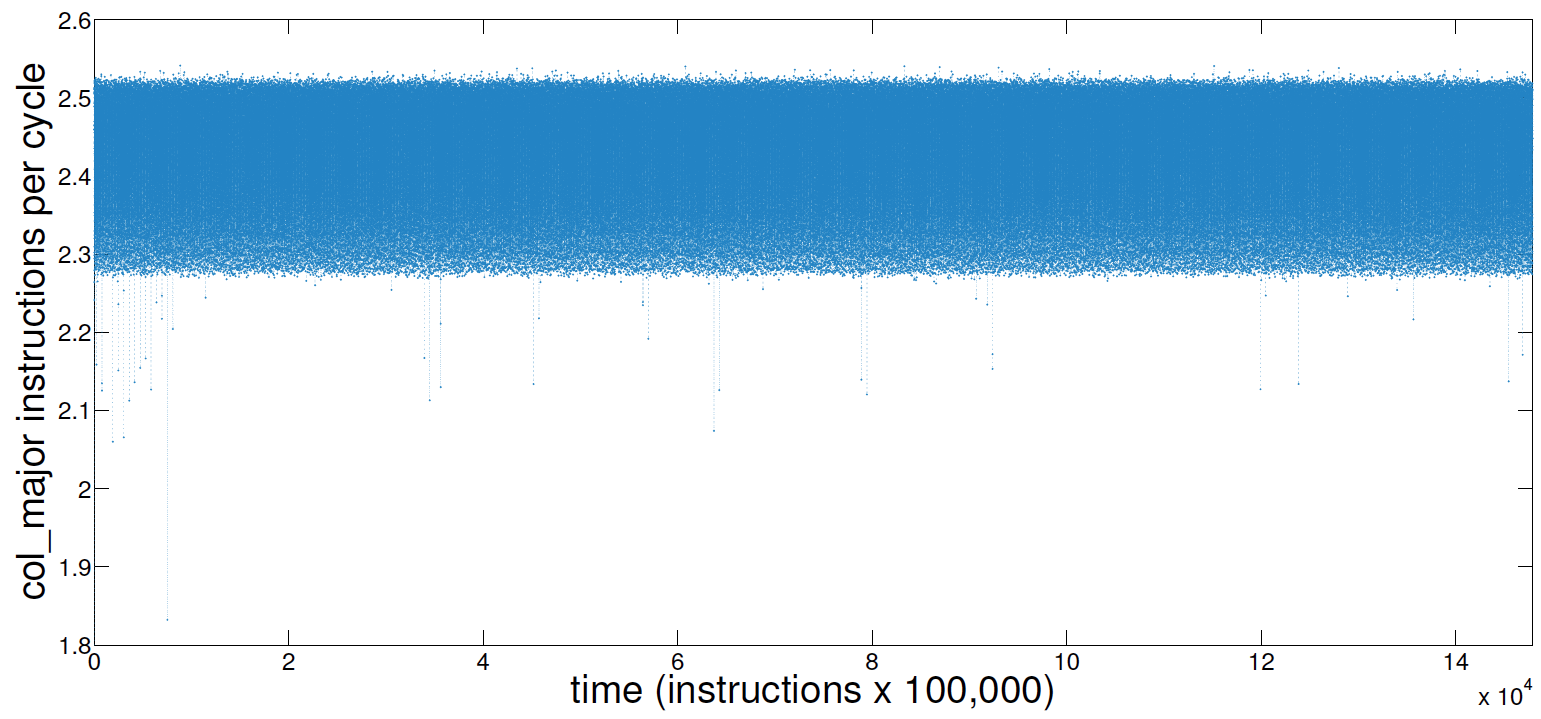
\includegraphics[width=0.95\textwidth]{figs/colFullTS}
    \caption{\col Time Series}
    \label{fig:col-ts}
  \end{subfigure}%
  \begin{subfigure}[t]{0.475\textwidth}
    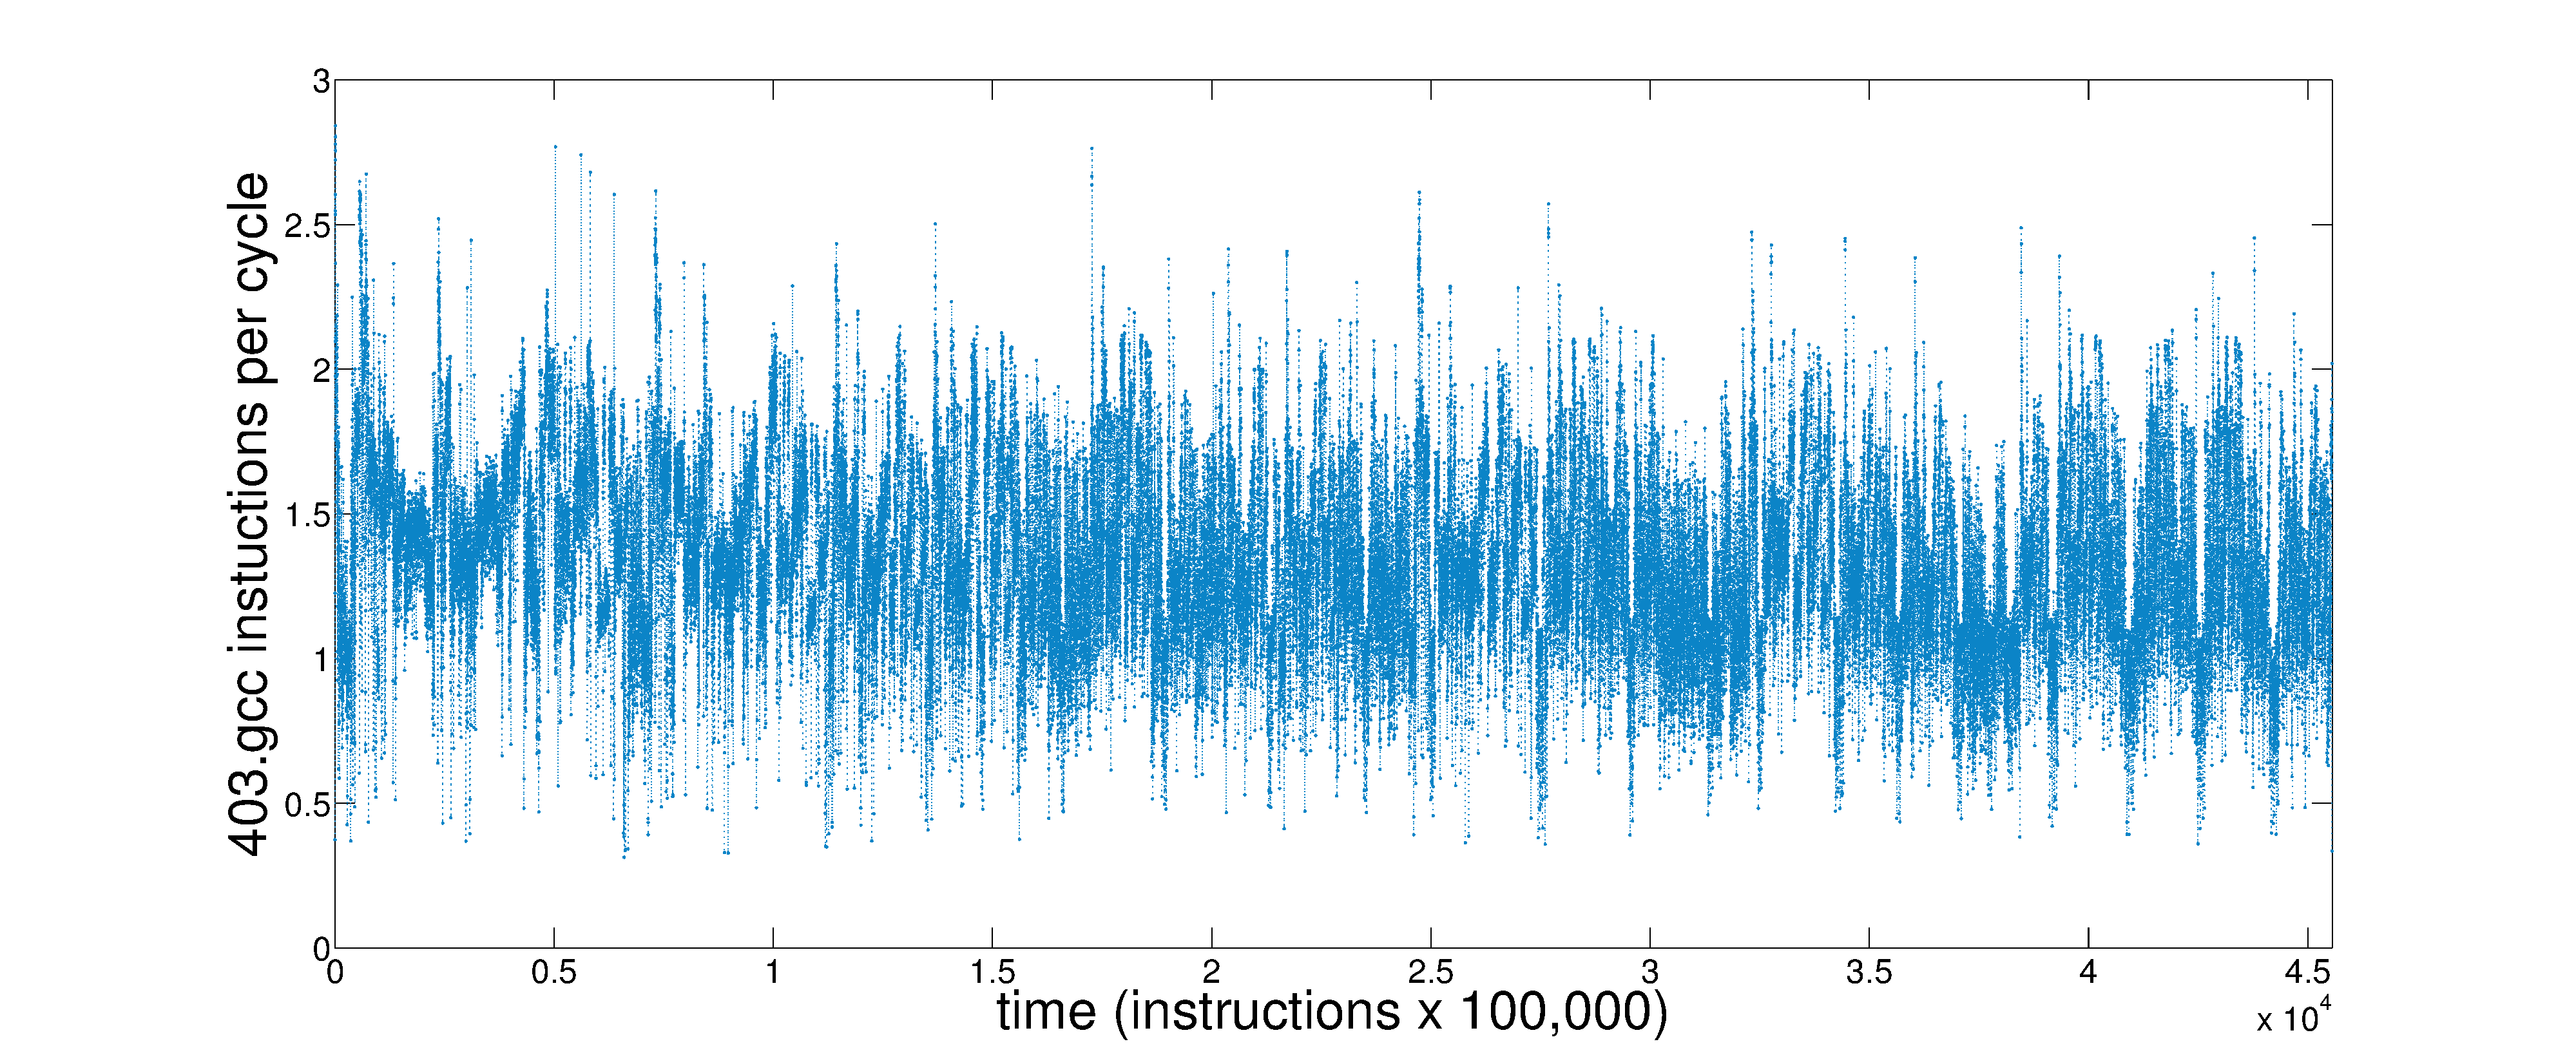
\includegraphics[width=0.95\textwidth]{figs/gccfullts}
    \caption{\gcc Time Series}
    \label{fig:gcc-ts}
  \end{subfigure}
  \caption{In (a) the instructions executed per CPU clock cycle
    (IPC) during the execution of \col. Each point is the average IPC during a 100,000
    instruction period. Similarly in (b) is a time series of the IPC during the execution of \gcc.}\label{fig:sample-ts}
\end{figure}
